\chapter{Approaching the Mountain}
\section{Entering the Valley}

My journey to document our blocky world has lead me to many different places. One that always tugs on my heart is the Bebbocraft Season 4 Valley and the impressive landmark at its center.
A kindly trader tipped me off to this beautiful valley during a trade we made while they were visiting my home. Having just passed through on their nomadic journey, they were delighted to tell me of its views after I lined their pockets. They said it was over the mountain range far to our north. Being the enterprising and daring adventurer that I am, and owing to my colonial ancestry, I began preparations for a journey to survey the new lands as soon as I could.

The mountains between me and my quarry were nothing to balk at. My plane needed a full slate of fuel and cold weather upgrades just to crest over the ridge more than once. In spite of this I persisted and was able to surmount the ridge to the valley a mere three weeks after learning of its existence.

The first view I was able to capture is from directly south on the morning that I entered into the valley. This was my first view of my new muse. Its prominence is immediately visible from the high vantage point on the ridge.

Low lying marshes dominate this area of the valley. The massive amounts of decomposing matter soak into the water and create an especially nutritious soup for the flora and fauna. I believe this to be the reason why vibrant cherry blossoms and orchids are so common in this section of the valley. Further research would be needed to confirm my theory. While the area is beautiful, I could not stand the constant incursions by mosquitoes. The crocodiles kept their evil eyes on me as well.

The second view comes from an island I took a break on not far from that ridge I crested in the morning. Its visible from the first shot as the island on the far right. The spit of land was positioned is where I first encountered the bright blue orchids that seem unusually common in this region. I named this island New Liverpool. Other than the mosquitoes, I quite prefer New Liverpool.

\begin{figure}[H]
    \centering
    \includegraphics[width=1.1\textwidth]{Cresting over the ridge into the Season 4 Valley Sunrise.png}
    \caption{Cresting over the ridge into the Season 4 valley at sunrise.}
    
\end{figure}

\begin{figure}[H]
    \centering
    \includegraphics[width=1\linewidth]{Isalnd down the ridge.png}
    \caption{Stopping for a pic in the orchid swamp.}
\end{figure}

\section{Encounters around the Base}

\large
As I got closer to the mountain, its prominence began to really register to me. While it doesn't quite reach the spectacular heights of the Scarlet Bebbonian Mountains to the northeast, or compete with the largest of the peaks on the southern Bebborian mountain range, it is notably prominent geographically. As long as you are in this valley, or one of the oceans bordering it, Mount Bebbo is always visible. Nothing natural comes close to competing in its shadow and the ranges nearest to it almost seem to be giving it a wide berth.

On a large plateau not far from the island I rested on, I spotted a small savanna. Dotting the plains were giraffes and elephants of numbers I had not see this far north. A constant warm breeze seemed to sweep out from the base of Mount Bebbo blanketing the grasslands. Perhaps that was the source of the warmth these animals needed.

Another theory gained credibility in my mind after I noted that Mount Bebbo is volcanically active. The whole valley seems to be covered in geothermal vents and lava pools. The mountain itself has multiple large and active lava flows that pour out new earth onto the base at all times. The rock making up the mountain is undeniably volcanic in nature and has a dark and brooding color. Especially when it is not covered in the white fluffy snow characteristic of the volcanically dormant faces of the mountain.

Perhaps the magma that once granted Mt. Bebbo its prominence also provides the temperature gradients necessary to support the diverse array of creatures that call this valley home. The magma probably even cleanses the water and infuses it with all sorts of wonderful natural minerals, like sulfur!

As I pondered hard on the nature of these things, I noticed a giraffe also partaking in the sight of Mount Bebbo. I knew in that moment that the beast was far wiser than I. It chose to savor a view that I could only think to dissect. Its ability to utter fewer words than I forever trumping me in the brevity part of the wit equation just as its simple mind let it appreciate nature's art far more primally than I ever could. 

\begin{figure}
    \centering
    \includegraphics[width=.9\linewidth]{Giraffe Ponders Bebbo.png}
    \caption{A lone Giraffe contemplates the nature of Bebbo.}
\end{figure}

\begin{figure}
    \centering
    \includegraphics[width=1.1\textwidth]{Bebbo In Full.png}
    \caption{The Base of the Bebbo climb.}

\end{figure}

\begin{figure}
    \centering
    \includegraphics[width=1\linewidth]{3 Little Birds Guide me up the Base.png}
    \caption{Three little birds greeted me during my ascent.}
\end{figure}

\chapter{The Summit and Beyond}

\section{Peak and Valley}

\large
Standing atop the peak I was overcome with euphoria at the discovery of this new land. Signs of the previous inhabitants were numerous. 

The closest sign of civilized life was just south of the peak. There a village rises from the plains. As I approached I noticed something as amiss about the village. Huge amounts of the land had been cleared and replaced with torches jutting from the ground. The grass was perfectly mowed and there wasn't a single living being in site.

Venturing closer I found that the settlement was completely abandoned. All of the structures with roofs were devoid of life. There was a strange encampment hewn from black stone on the outskirts as well. The encampment was extremely well stocked and in good condition for being exposed to the skies. I would have inspected the area closer but I swear I began hearing voices come from the ground. Columns of water seemed to carry the sound upwards but I dared not inspect the source. Maybe on a future expedition.

\begin{figure}[H]
        \centering
        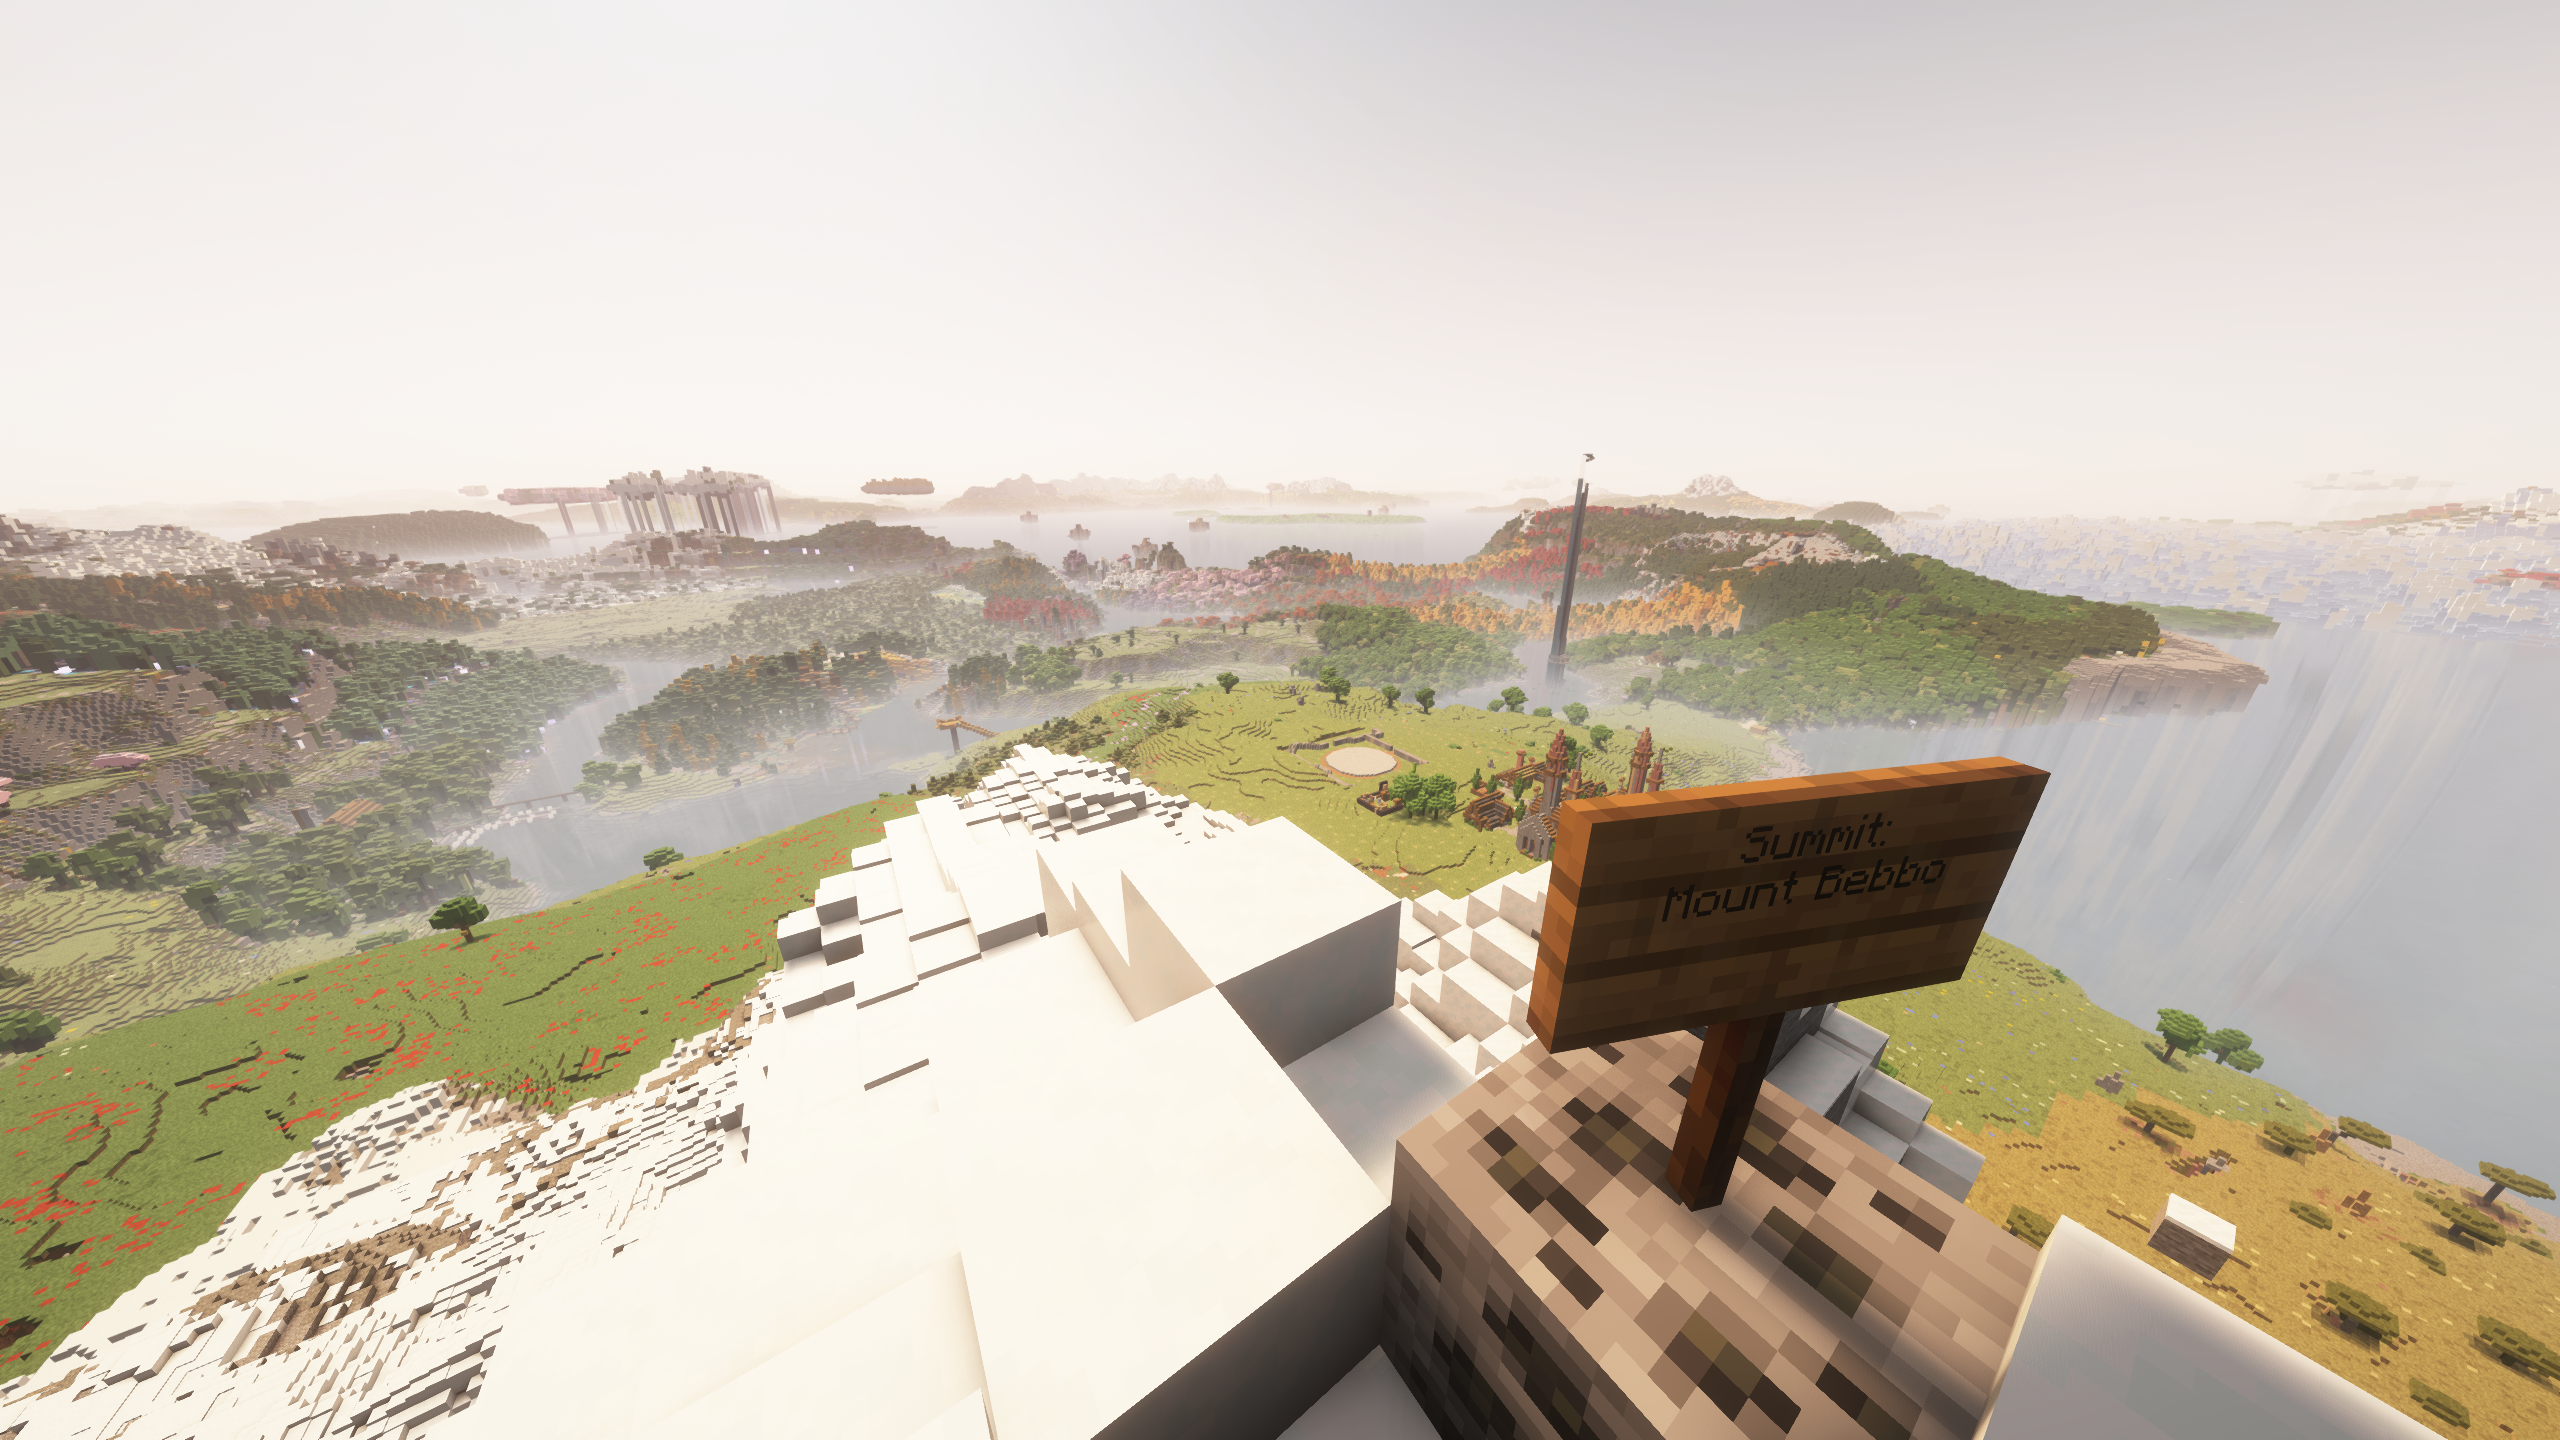
\includegraphics[width=1\linewidth]{View from the Summit.png}
        \caption{The Summit of Mount Bebbo.}
    
\end{figure}

\begin{figure}[H]
    \centering
    \includegraphics[width=1\linewidth]{The light square from on Mount Bebbo.png}
    \caption{The Light Square.}
\end{figure}

\begin{figure}[H]
	\centering
	\includegraphics[width=1\linewidth]{Ghost Town.png}
	\caption{An Abandoned Village.}
\end{figure}

\section{Signs of Life}

\large
Travelling away from the site of the torches I came upon more signs of civilization. A tower reaching far into the sky sat in the middle of a river that runs through this section of the valley. Water continually flowed from the top and poured back into the river it was pumped from. I would regard this structure as a fountain but this is far larger than any fountain I know of. This valley was already filled with so much wonder and I had barely just begun. Surely, I was not alone out here.

Up the hill from this tower was a structure seemingly called the "Spawn Cabin". It was very well furnished but I dared not stay long. The stillness of the air felt like an omen. A portent that I would not be able to leave if I stayed too long. I do not know what kind of spawn reside in this cabin but I was not intending to find out. 

As I took the photograph from behind the cabin, I was greeted by one hell of a man, named Bebbo. He said he was the "Admin" of the area but he seemed more like a king to me. After a brief pleasant conversation, this towering figure of hospitality took me by the hand and whisked me away. In front of the cabin we plunged and explored depths I could never have imagined. He slammed me into a cart and everything began moving so fast. Before I knew it we were rocketing to the top and came out of the hole, soaked.

As we dried ourselves off he showed me the view out of his window. An avid aviator just as yours truly, he had built a runway facing the mountain. As we made our way to his hangar, he showed me a deep mine shaft he had constructed into the earth. He warned me that it had intersected the ruin of an ancient civilization with a monster most dangerous. I decided to avoid delving down, at this point my mission had become to photograph the mountain in all its glory. So we meandered to the taxiway, hopped in our aeroplanes, and set off for our first destination.

\begin{figure}[H]
	\centering
	\includegraphics[width=\linewidth]{The Tower.png}
	\caption{The Fountain Tower}
\end{figure}

\begin{figure}[H]
	\centering
	\includegraphics[width=\linewidth]{From behind spawn.png}
	\caption[]{A View behind the Spawn}
\end{figure}

\begin{figure}[H]
	\centering
	\includegraphics[width=\linewidth]{View from Bebbo's House.png}
	\caption{Bebbo's Abebbode}
\end{figure}

\chapter{A Grand Tour}

\section{To the North}

We travelled a short way due north to arrive at the site of a new dwelling under construction. Standing atop a large hill, the structure was on one of the highest hills around Mount Bebbo and was dotted with hot springs. This base belonged to a being known only as Jim. We did not linger long as we still had the longest leg of our journey to go.

Our next stop was a large alpha biome island to the northwest. Bebbo warned that a vast ocean stood between us and our next goal. It took most of a day just to cross with high speed aeronautical craft. We soared over countless pirate ships, some of whom tried foolishly to fire upon us. The sheer lawlessness of it all was staggering to behold. Although it does not suit my noble character, I do wonder if I could have been a privateer. I used to be quite proficient with a cutlass in my early youth and the pirate getup would be quite dashing on me. I think I would call myself Starchey.

The next stop's settlement was quite grand in nature. Active construction sites dotted the island it was on. There appeared to be a wholy new town being constructed from the thin air! In the center of the settlement stood a grand chateau where we met the leader, Ben. He offered us lodging for the night and a tour, which we happily accepted. Explaining to us as we walked, Ben told us of how this was meant to be a place of welcome. Somewhere new settlers could get started without needing to fully brave the elements on their own. At the end of the tour I captured an image of Ben looking to the now very distant Mt. Bebbo. He treated us to a meal and let us rest.

\begin{figure}[H]
	\centering
	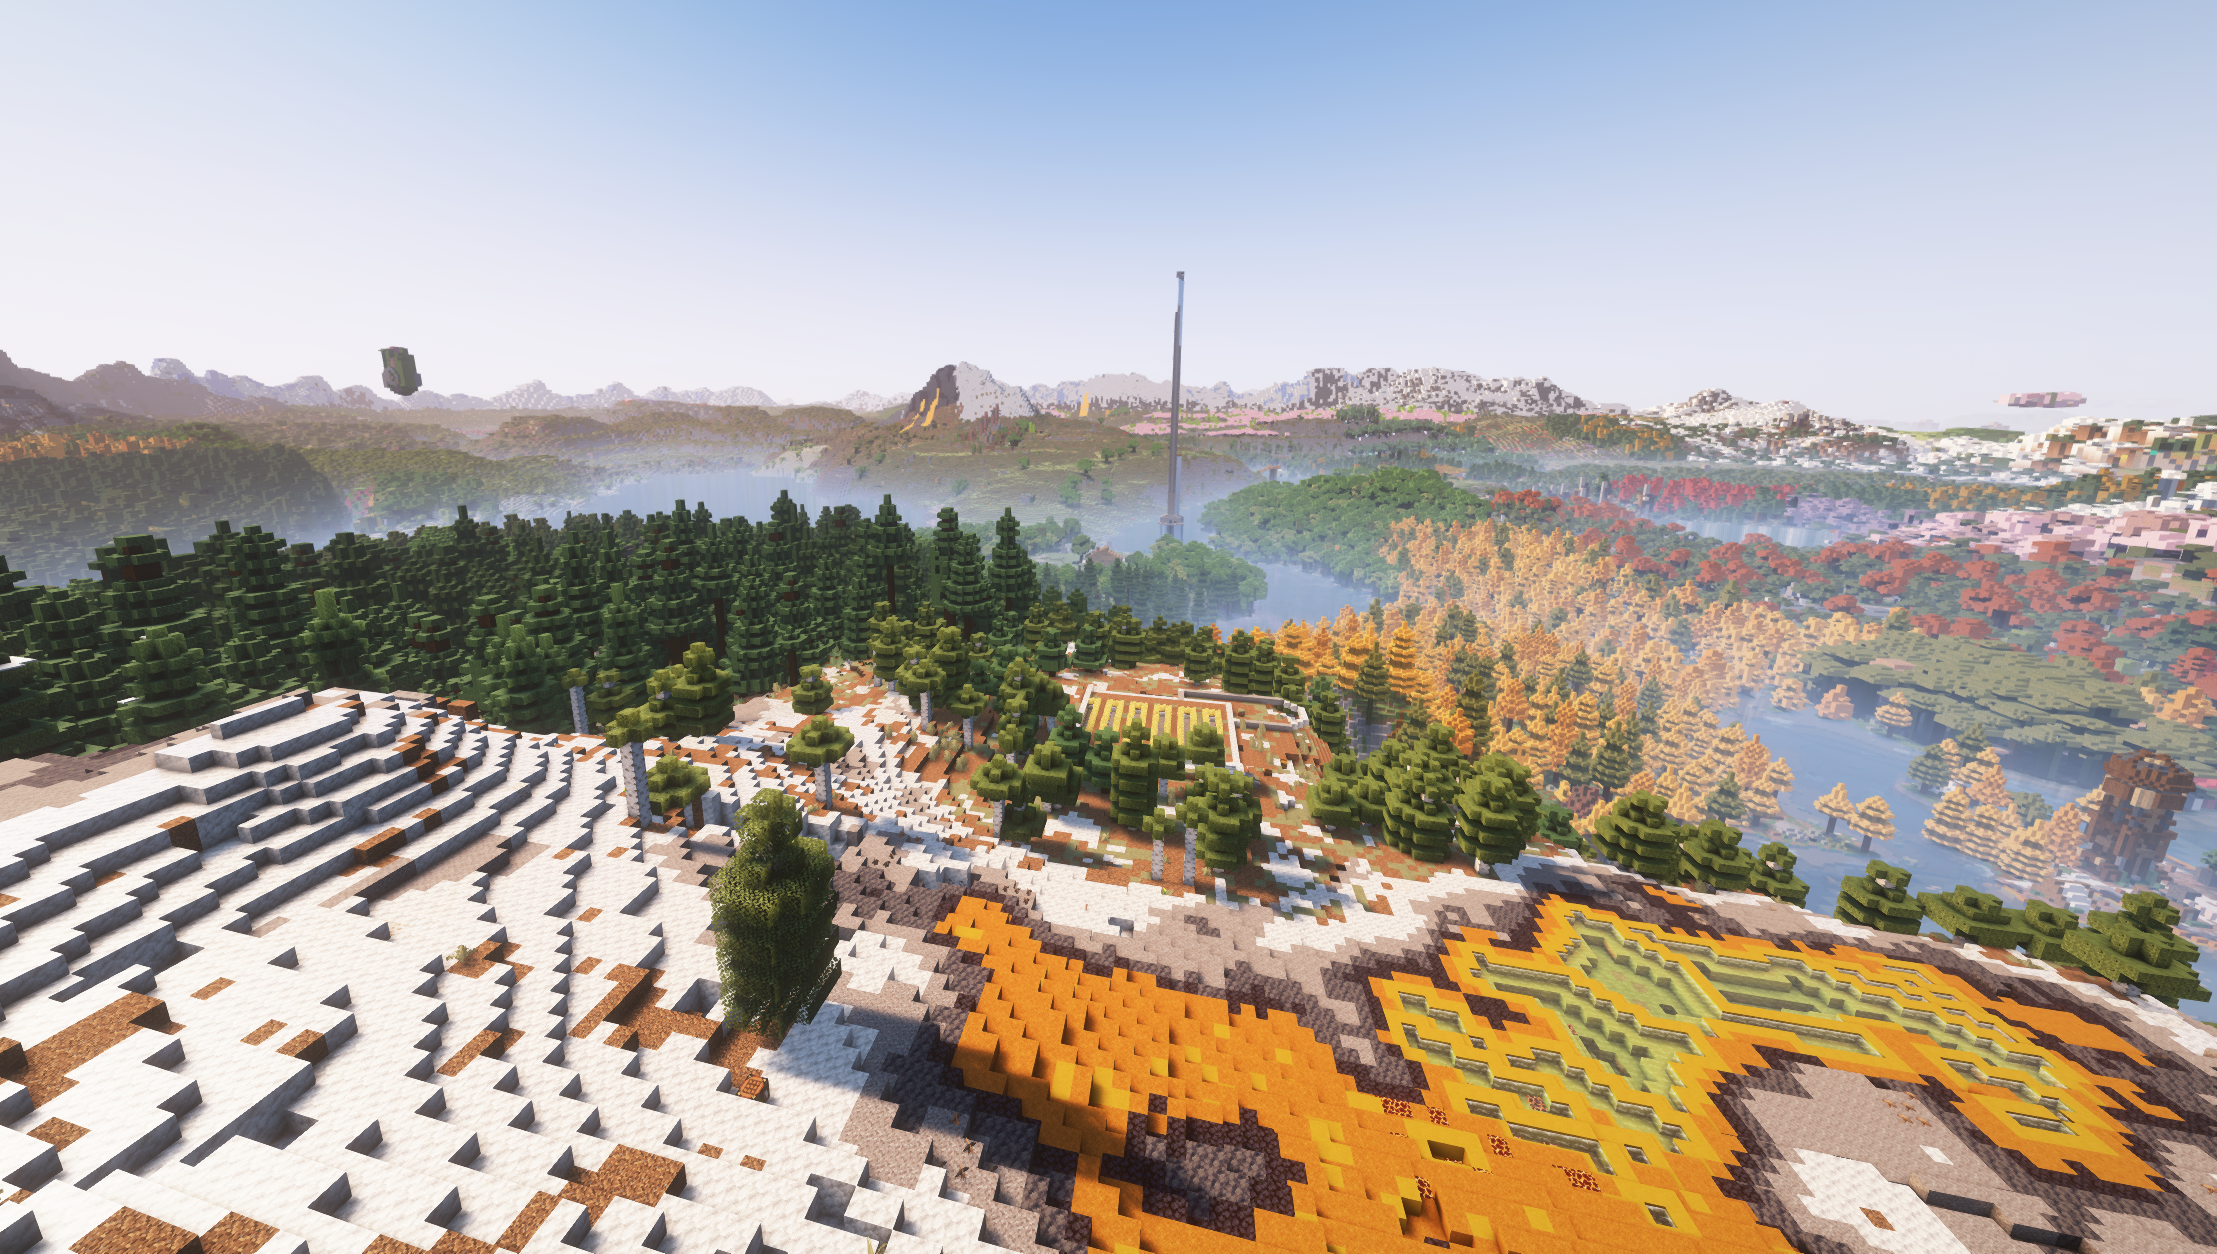
\includegraphics[width=\linewidth]{Hot Springs at Jim's.png}
	\caption{Hot Springs on a High Hill}
\end{figure}

\begin{figure}[H]
	\centering
	\includegraphics[width=\linewidth]{Guard Tower on Alpha Island.png}
	\caption{Guard Tower on Alpha Island}
\end{figure}
\newpage
\section{To the South}

We set off from Ben's island continuing our journey to the occupied lands south of Mt. Bebbo. Once again we crossed the buccaneer filled seas. The land looked so peaceful from high above. You can barely see the individual creatures from high enough up. The world begins to merge into a single connected painting. Every stroke of mountain, splash of forest, and setting of river further improving on a work of art only nature could create.

The voyage was long enough that we needed to camp for the night on the banks of the river valley. I captured these interesting sunset and night views of the mountain from the area around there after we set up camp. I find it interesting how the lighting and weather change the character of the mountain. It looks inviting one minute, calm the next, dangerous another, and majestic all throughout. I find myself compelled to include it in everything I do around here.

The next morning we set off to tour the last of the bases. We passed a few unfinshed bases before we arrived at the first stop. A dock with a tugboat stood just off the shore of a base still needing a roof. The boat concealed a drop deep into a base below the earth. Hewn blackstone, tarnished copper blocks, and a garage filled with books decorated this abode below the earth. After inspecting the room for a bit, we were startled to see that skeletons began falling from the ceiling into a cage. Within a couple minutes, there were hundreds of these skeletons. The clattering of bones became too much and we escaped through the water elevator before any of the rattlers clattered onto the floor through the cage.

Our next stop was a mangrove swamp. Out front floated a runway and set of docks for visitng this base. Up the stairs from the runway was a concert hall standing near a tent filled with supplies. Following the paths through the dense swamp revealed a train station and a stairway heading up to the top of the hill. From there was a beautiful view of Mount Bebbo, pictured both here and on the cover of the book.

\begin{figure}[H]
	\centering
	\includegraphics[width=\linewidth]{Sunset by the River Valley.png}
	\caption{Sunset by the River Valley.png}
\end{figure}

\begin{figure}[H]
	\centering
	\includegraphics[width=1.1\linewidth]{Rain At Night in The River by Mount Bebbo.png}
	\caption{Rain At Night in The River by Mount Bebbo}
\end{figure}

\begin{figure}[H]
	\centering
	\includegraphics[width=0.6\linewidth]{Tugboat.png}
	\caption{Bebbo Between Boat and Hook}
\end{figure}

\begin{figure}[H]
	\centering
	\includegraphics[width=\linewidth]{hills Near Bebbo.png}
	\caption{Climbing the Stairs in the Swamp}
\end{figure}
\newpage
\section{Heading out of the Valley}

At this point we only had a single stop left on the tour. Two of the newer residents to the valley set up an outpost on a ridge far to the south. They clearly are animal lovers as the pens outside their house were filled to the brim with all manner of livestock. The view was quite nice.

It was at this point that my guide Bebbo needed to return to his duties. I thanked him for his boundless generostiy and steady companionship. His efforts are what made this whole journey possible. We shared a short embrace before I watched him fly off towards the mountain that was his namesake.

Now at the end of my maiden voyage to the valley, I decided to climb the ridge I came over when I first arrived. I reached the peak just as night reached a peak of its own. It was here that I was gifted with one final spectacular view of the mountain. An Aurora came into view over the valley and left me speechless. It was the perfect end to my journey.

\begin{figure}[H]
	\centering
	\includegraphics[width=\linewidth]{Juans base.png}
	\caption{Juan and Cassidy's base}
\end{figure}

\begin{figure}[H]
	\centering
	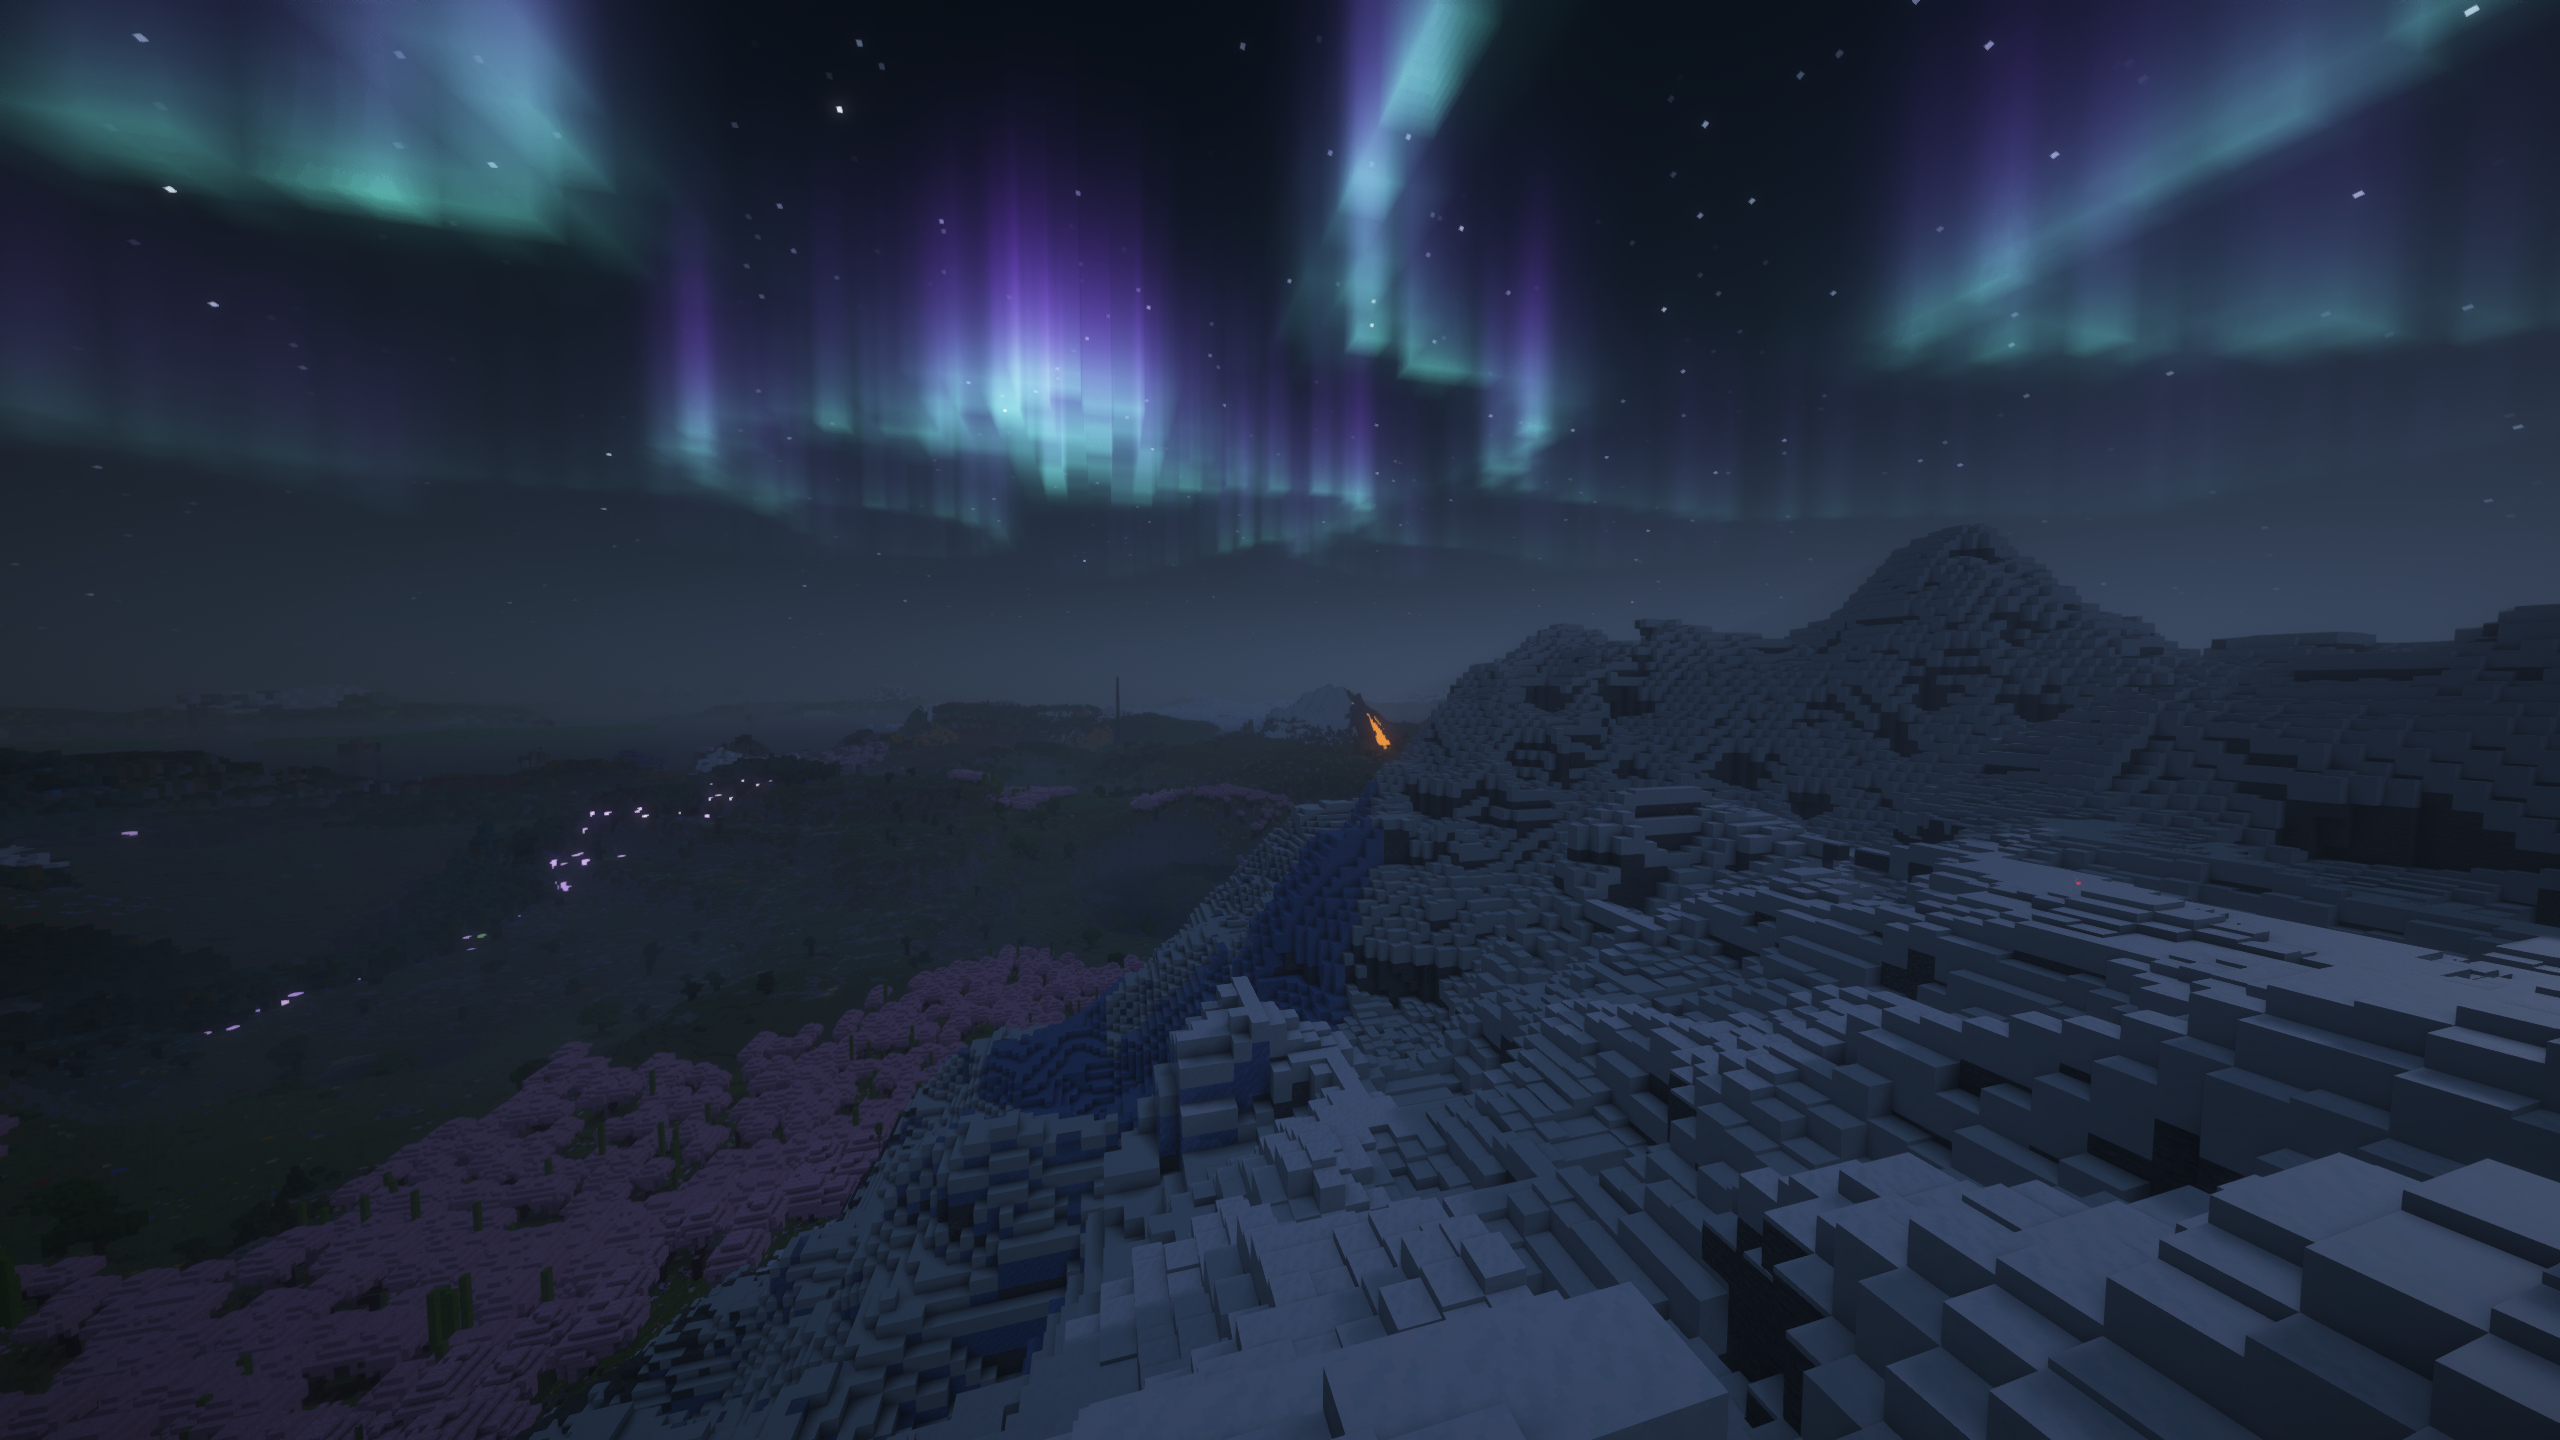
\includegraphics[width=\linewidth]{Aurora over Mount Bebbo.png}
	\caption{Aurora over Mount Bebbo}
\end{figure}

\chapter{Views from my Own Explorations}

Here is a collection of views that did not fit into the other chapters, or came from later expeditions. All are included because I felt they captured an aspect of the mountain that was not explored in another image from the book.

To say that the journey's to and from Bebbocraft valley have changed my life would be an understatement. I hope everyone gets to experience a place in their life that makes them feel as awe filled and serene as I feel when I can see Mount Bebbo. 

Mount Bebbo is clearly a landmark most holy and of utmost importance. I hope this book serves as a glowing review. Everyone should visit if they have the means. Consider it a pilgrimage. 
\begin{figure}[H]
	\centering
	\includegraphics[width=\linewidth]{Bebbo Under Moonlight.png}
	\caption{Bebbo Under Moonlight}
\end{figure}

\begin{figure}[H]
	\centering
	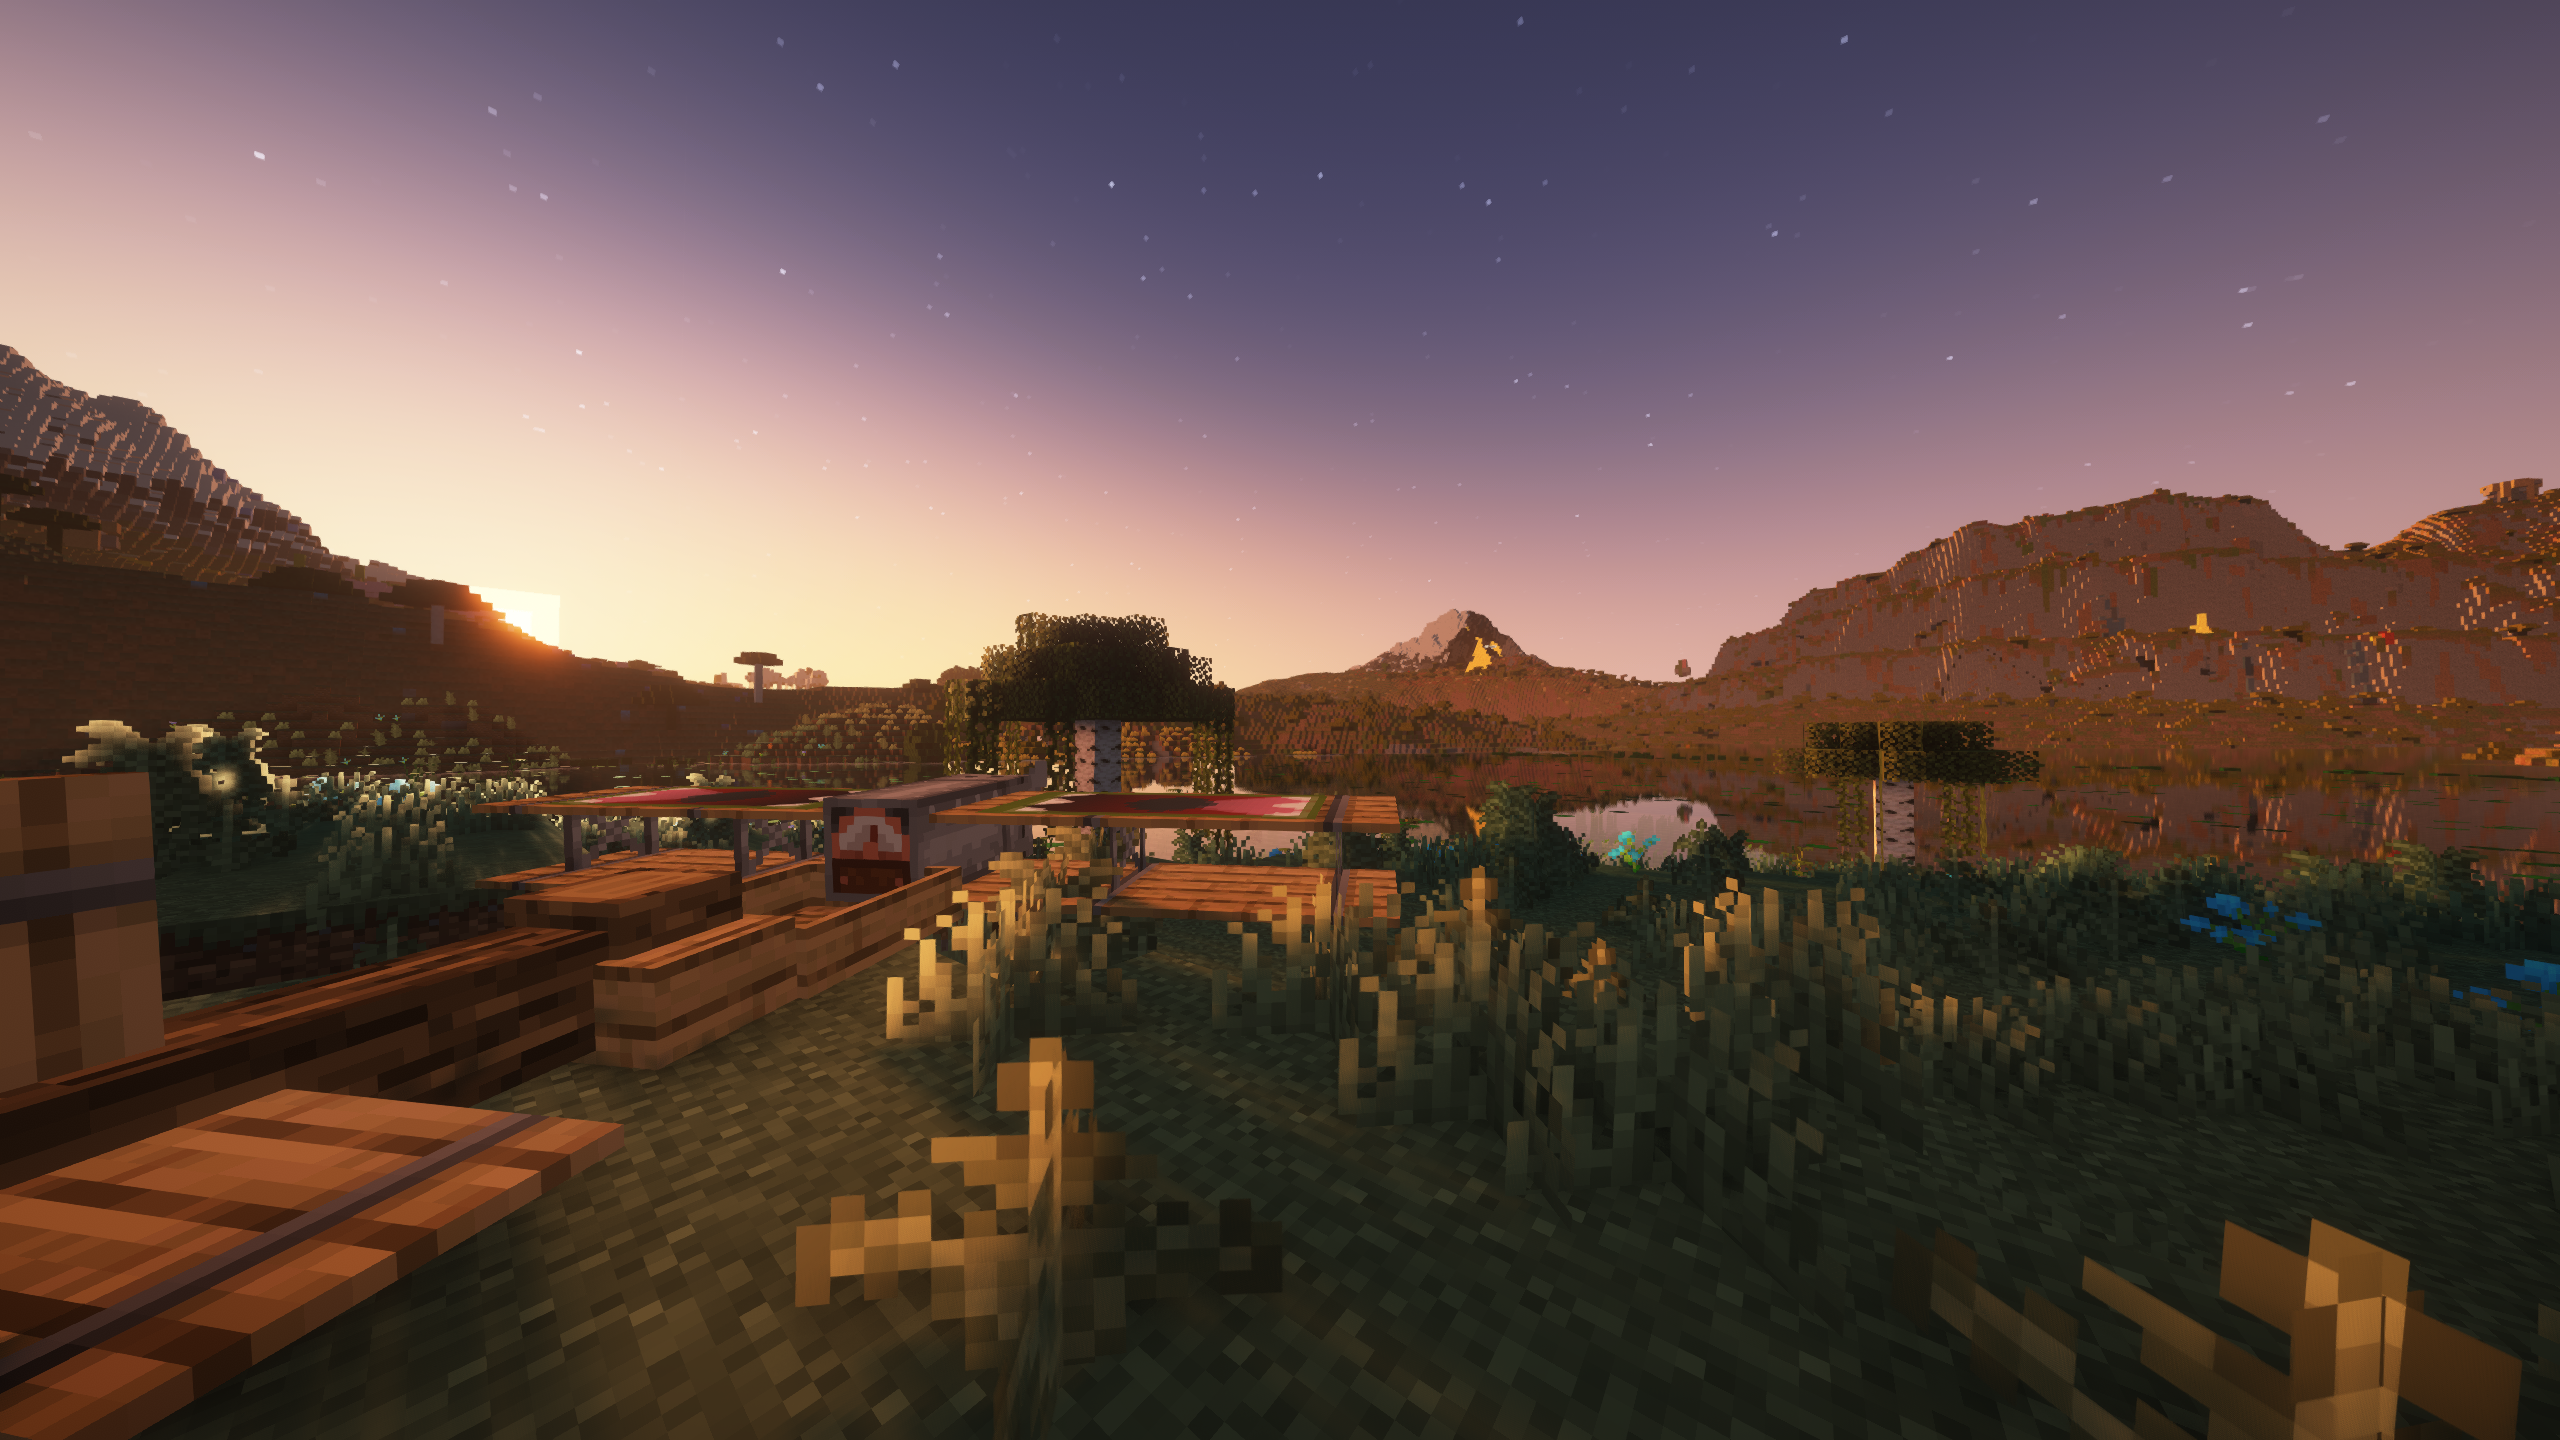
\includegraphics[width=\linewidth]{My Trusty Companion.png}
	\caption{My Trusty Companion}
\end{figure}

\begin{figure}
	
	\begin{subfigure}[t]{0.3\linewidth}
		\centering
  	  \includegraphics[width=0.5\linewidth]{Biplane over Mount Bebbo at Night.png}  % Replace with your image file 
	\end{subfigure} %

	\begin{subfigure}[t]{0.3\linewidth}
		\centering
   	 \includegraphics[width=0.7\linewidth]{Biplane over Mount Bebbo at Sunset.png}  % Replace with your image file
   	 
	\end{subfigure}
	\begin{subfigure}[t]{0.3\linewidth}
		\centering
		\includegraphics[width=1.5\linewidth]{Mount Bebbo from 10KM.png}  % Replace with your image file
	\end{subfigure}
	\caption{A collection of views far above the ground. Note Mount Bebbo in all.}
\end{figure}

\begin{figure}[H]
	\centering
	\includegraphics[width=\linewidth]{Cresting over the ridge into the Season 4 Valley.png}
	\caption{Cresting over the ridge into the Season 4 valley at sunset.}
\end{figure}

\begin{figure}[H]
	\centering
	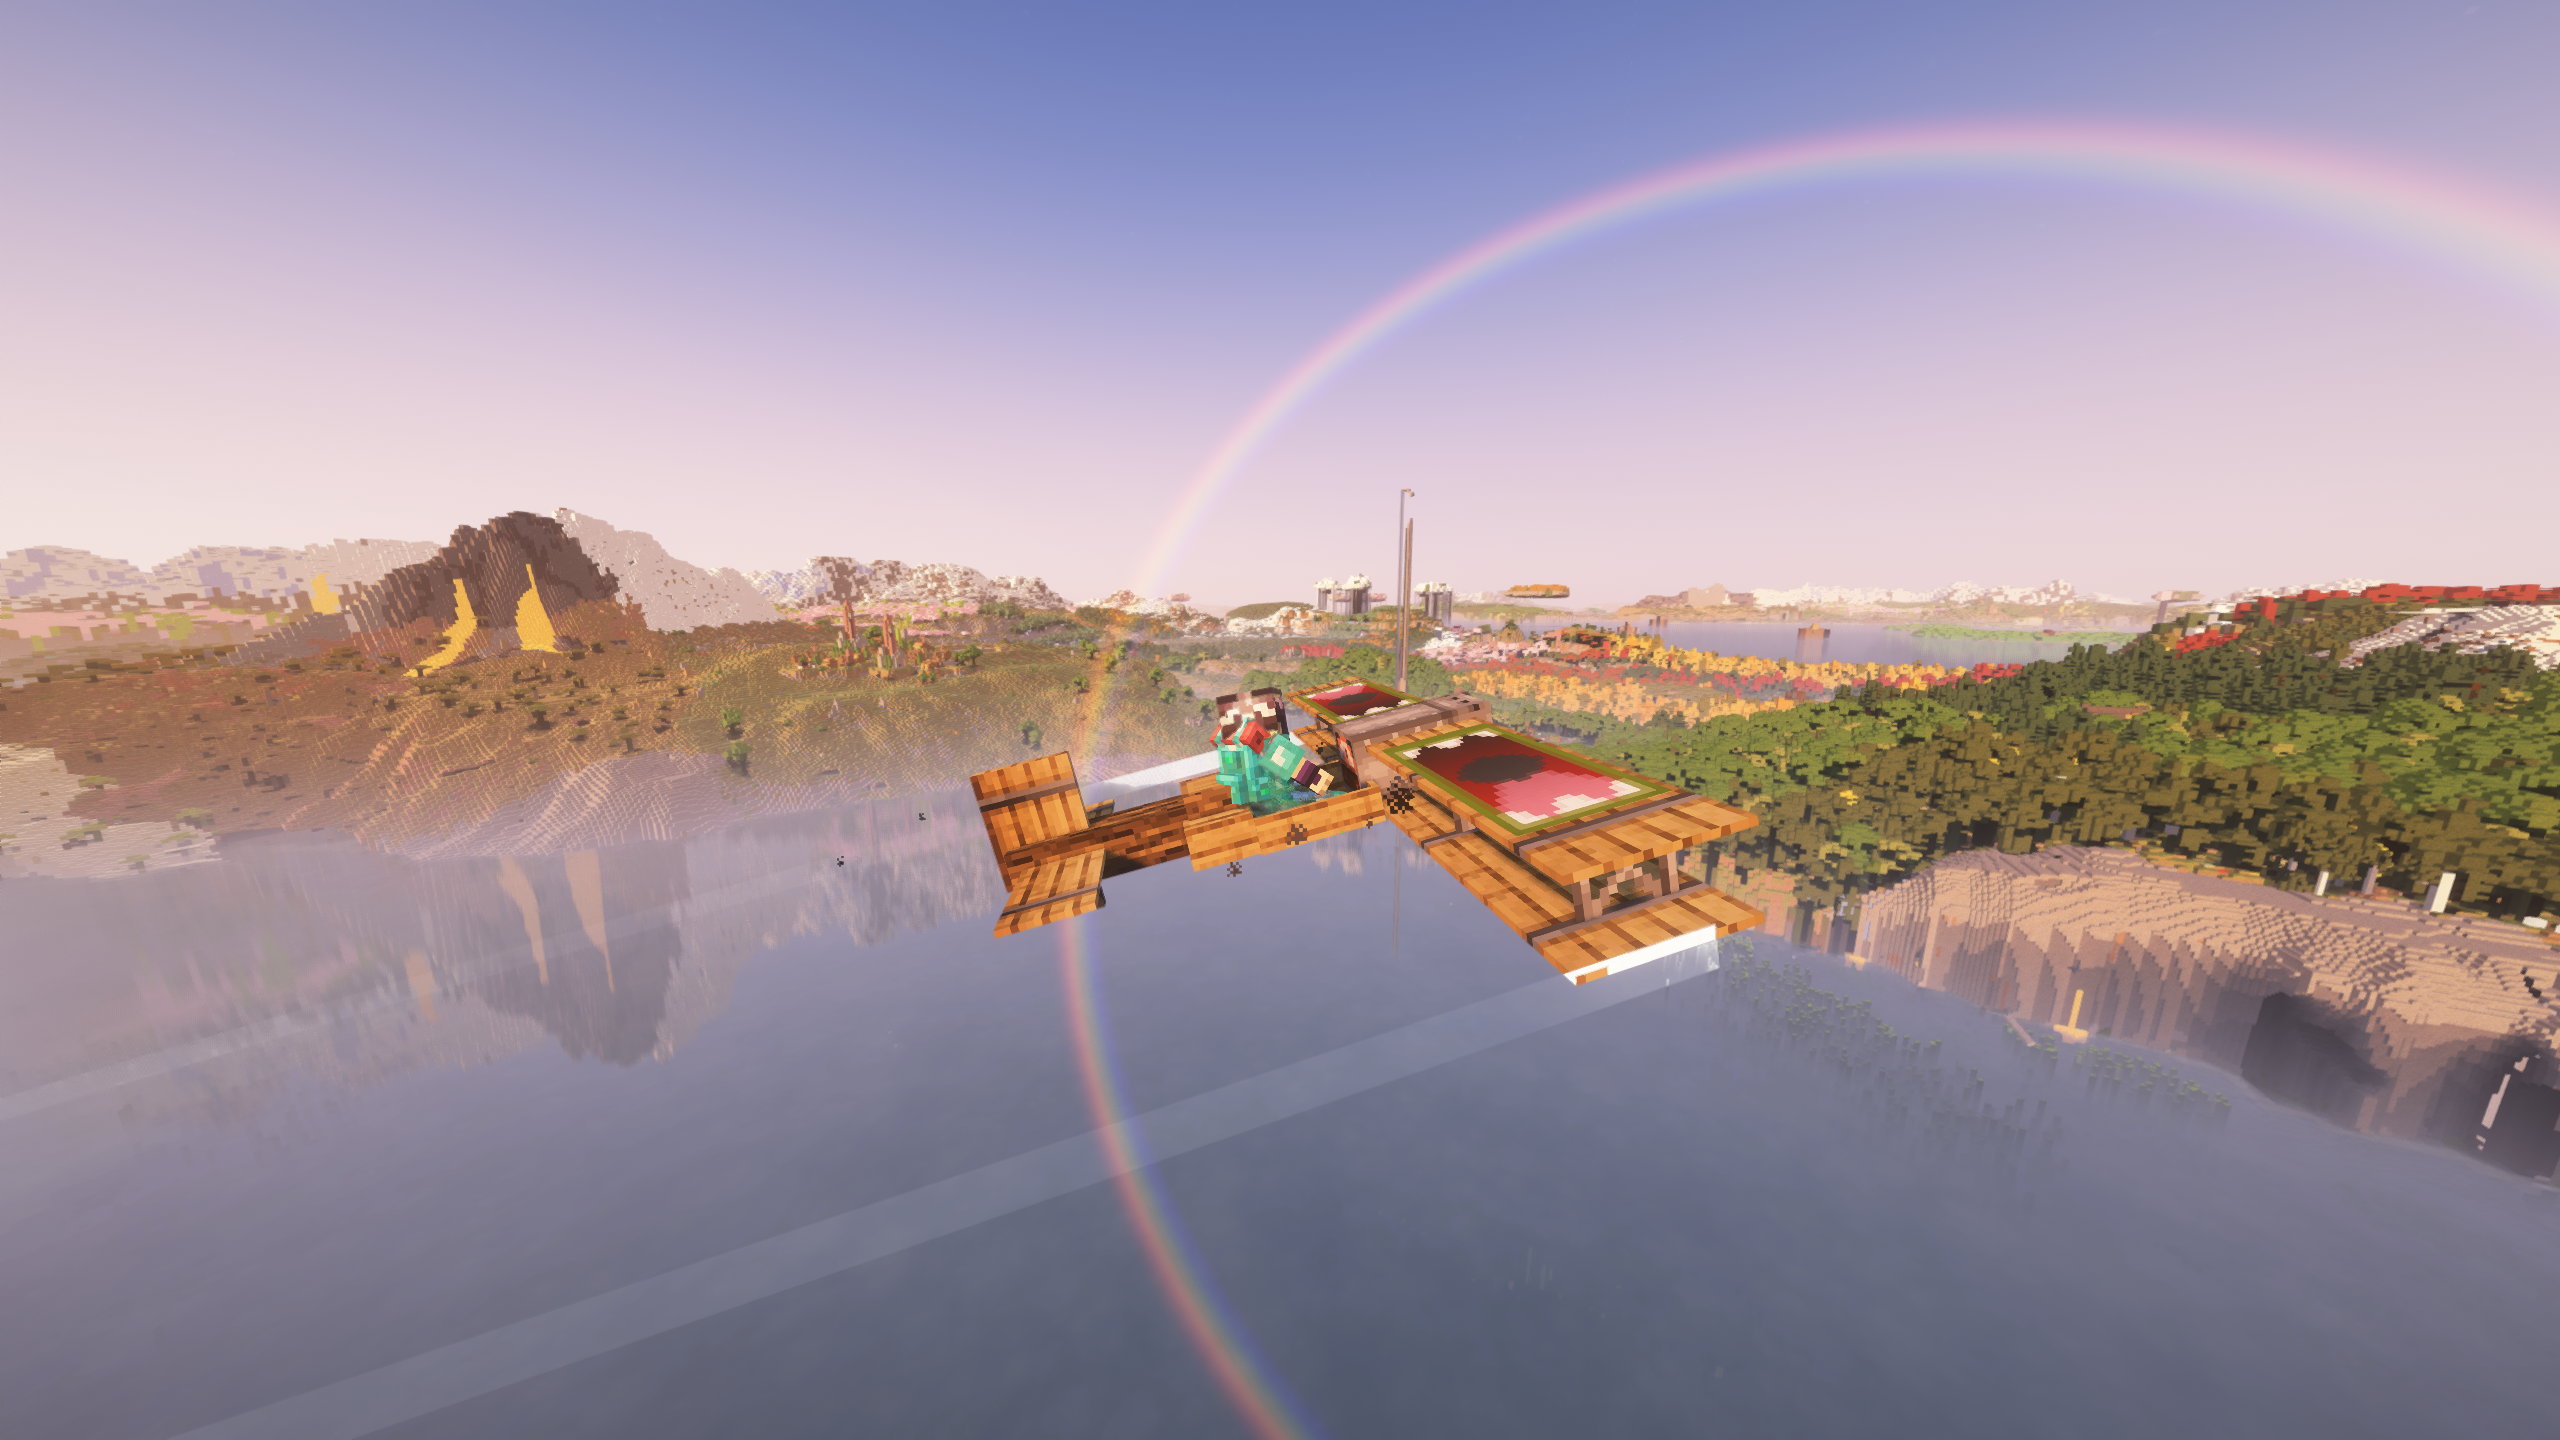
\includegraphics[width=\linewidth]{Rainbows near Mount Bebbo.png}
	\caption{Rainbows near Mount Bebbo.}
\end{figure}

\begin{figure}[H]
	\centering
	\includegraphics[width=\linewidth]{Day View of Mt Bebbo.png}
	\caption{Diurnal Bebbo.}
	
\end{figure}
\newpage
